\chapter{Background knowledge}

In this chapter, I will put some basis, and explain some concepts related to my work.  Reading this chapter should allow the reader to understand what I did in this work, supposing he is already familiar with Linux.

\section{Virtualisation, Containerisation, Runtime isolation}
\paragraph{}We always have the same goal: being able to execute some code, with no interaction with someone else's one.  As of course, we cannot use one bare-metal machine for each application we want to run, some mechanism has to be used to provide isolation between coexisting processes on the same physical machine.

We can distinguish three level of isolation: Virtualisation, Containerisation and Runtime isolation (Figure \ref{fig:virt-cont-runt}).
\begin{figure}
  \begin{center}
    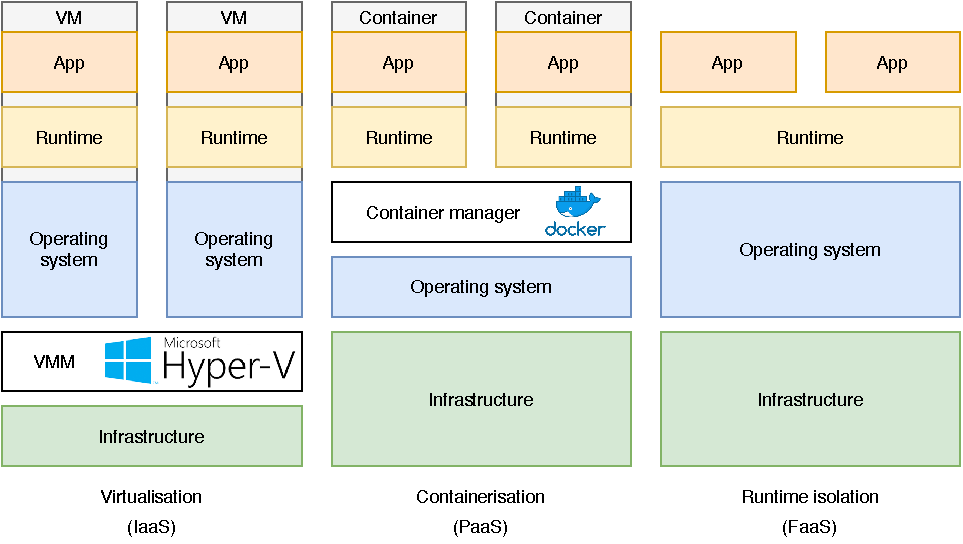
\includegraphics[width=\linewidth]{images/Virt-Cont-Runt.pdf}
    \caption{Different isolation level for an application.}
    \label{fig:virt-cont-runt}
  \end{center}
\end{figure}
\subsection{Virtualisation}
The isolation layer is located either between the hardware and the guest OS (hypervisor of type 1) or between virtualization of the hardware and the guest OS, with a hypervisor (type 2) running in another OS.  In both cases, the guest OS will run as if it was on a bare-metal machine, executing its kernel, managing its drivers, its file system, etc.  This is the stronger isolation we can get.  Cloud providers can rent you some Virtual Machines, this is what we call IaaS (Infrastructure as a Service).  You can use many different hypervisor solutions. Usually, Cloud providers have their very own solution.
\subsection{Containerisation}
Here we go one level higher: the isolation layer is located between the OS and the guest application.  This isolation mechanism is called a container, and is a set of processes, running in common namespaces, with a root filesystem different from the host.  Containers share the same kernel as the host though, which means that a process running in a container can be seen from the host.  Containers belong to the world of PaaS (Platform as a Service), a system where Cloud providers offer you to run your application (that you provide under a containerized form) without having to worry about all the infrastructure that needs to be deployed along with it, and sometimes even with some great scalability mechanism support.
\subsection{Runtime isolation}
This is the highest (weakest) level of isolation you can get.  The isolation is provided by the runtime on which the application is running (ex: The JVM for a Java program, a Python environment, ...).  Multiple guest applications share the same OS, file system, without any mechanism to hide it from them.  Cloud providers propose such service under the name of FaaS (Function as a Service).  For this, you can provide a small program, that you want to be executed on demand.  Cloud providers usually allocate a container to this program, to provide safer isolation, but will execute multiple instances of this program in the same containers, to avoid the overhead of creating a new container each time.  The type of programs you usually run in these is computationally intensive parts of your application. These need to have low response time and great scalability (for example resizing of user-uploaded images).  This model is often referenced as the Lambda model (from Amazon Lambda service) or as serverless computing.

\subsection{INGInious specific case}
The case of INGInious is a special one.  The type of the workload caused by the evaluation of the tasks (fast response time, varying demand, potentially big computation, logic independent of the core application) would suggest using a serverless strategy, but the isolation requirement are those of PaaS (as the various inputs of the functions are code of student to safely execute, isolated from one another).  Currently, the application relies on IaaS, running in multiple VMs where are hosted the core application and multiple docker agents.  

\section{Containers}
The isolation being the most important requirement, we will then look into containerization solutions: presenting the main concepts behind containerization, the global container ecosystem, the current solution that INGInious uses and the alternatives we have.

\subsection{Core concepts}
Containers rely on three components: namespaces, control groups and chroot.
\paragraph{}\textbf{Namespaces} are a feature of the Linux kernel since 2002.  A namespace can be associated with a context, which is a partition of all the resources of a system that a set of processes has access to, while other processes cannot.  Those sets of resources can be of seven kinds:
\begin{itemize}
\renewcommand\labelitemi{--}
  \item \textbf{mnt} (Mount): This controls the mount points.  Processes can only have access to the mount point of their namespace.
  \item \textbf{pid} (Process ID): When processes are in a pid namespace, the latest hides from them all the processes that are not in it.  The assignment of pid as seen by the processes inside the namespace is independent of the rest of the system.  The first process in the namespace will be the pid 1, the second, 2, etc.  From a parent pid namespace though, those processes can be seen, and have another pid (obviously pid 1 and 2 are already taken).
  \item \textbf{net} (Network): This provides a virtualized network stack.
  \item \textbf{ipc} (Interprocess Communication): This allows processes of the same namespace to communicate with one another, for example by sharing some memory.
  \item \textbf{uts} (Hostname): This allows to have different hostnames on the same machine, each hostname being considered as unique by the processes of its namespace.
  \item \textbf{user} (User ID): This allows to change the user id in a namespace.  This way you could have a user root in the namespace, which is unprivileged outside of it.
  \item \textbf{cgroup} (Control group): This allows to change the root cgroup directory. This virtualizes how process's cgroups are viewed.
\end{itemize}

\paragraph{}When a Linux machine starts, it initiates one namespace of each type in which all the processes run.  The processes can then choose to create and switch namespaces.

\paragraph{}\textbf{Control groups} are a feature of the Linux kernel that allows limiting and controlling the resources allocated to some processes.  You can for example control the CPU usage, the memory consumption, the io...  Recently (since kernel 4.5) a new version of cgroups (cgroups v2) appeared, which comes to tackle the flaws of the original implementation while keeping all of its functionalities.  The main change is the use of a new unified hierarchy to manage the control groups, where all the resources are centralized and where the allocation of some resources is done by adding a sub-resource-group in the hierarchy the current user has access to.
However, the adoption of the newer version is a process and takes time. Still now, many applications use the original version of cgroup.

\paragraph{}\textbf{Chroot} allows us to change the root of the root filesystem for some processes.  For example, we could create a directory \texttt{/tmp/myroot/} which contains all of the usual directories present in the original root folder (\texttt{/}) and set this as the new apparent root for the chosen processes.  This is not a complete sandbox, and not real isolation on its own, files from outside of the chroot could still be accessed.

\subsection{Storage drivers}
When it comes to handling a container file system, different solutions can be used.  The goal of each is to provide the most efficient writable root directory (\texttt{/}) for each container but keeping each container unaffected by the modification done in the other containers.

\paragraph{} To do so, three main strategies can be used:
\begin{itemize}
\renewcommand\labelitemi{--}
  \item \textbf{Deep copy}: for each container, the whole image is copied during the creation of the container.  This is simple but gets excessively slow as the file system size increases.
  \item \textbf{File based copy on write}: for each container, will be copied only the files that are edited during the container life cycle.  This is more complex but gets more efficient as the container's size grows.
  \item \textbf{Block based copy on write}: for each container, will be copied only the blocks (in the filesystem) that are edited during the container life cycle.  This is even more complex but get more efficient as some small part of big files are edited.
\end{itemize}

\paragraph{}Containers are a specific kind of workload in the sense that a lot of information, data, is redundant in different containers.  For example, for a simple application, we could use several containers with different responsibilities and tools embedded in it, but all based on the same Alpine image.  This brought a new space problem, as we do not want to avoid duplicating too much data.  To face this, \textbf{union filesystems} are used, along with layered container images.  This means that different container images but with the same basis will share the common part of their file system, avoiding the need to duplicate it.  It differs from the file system deduplication mechanism by the level at which the action is taken.  For deduplication, when a block is written on disk, we check if similar data is not already located somewhere.  Whereas for a union file system, the common base image will be read-only, and when an attempt to modify a file is made, a bind mound will be made with a copy of the file on top of the original one, so that the common base stays preserved.

\paragraph{}The storage of a container has to be backed by a file system, which will eventually already provide some interesting mechanisms for the container.  Those four main filesystems used are:
\begin{itemize}
\renewcommand\labelitemi{--}
  \item \textbf{BTRFS}, presented in 2013, \cite{rodeh2013btrfs} is a general-purpose file system, based on copy-on-write and with efficient snapshots capabilities and strong data integrity.
  \item \textbf{zFS} is similar to BTRFS (but was there before), but handles some mechanisms differently, like the management of blocks (blocks vs. extends\footnote{zFS can have blocks to up to 128KB, while BTRFS will only use the extend strategy (point to the next block).}), snapshots (birth-times vs reference-counting\footnote{When doing snapshots, zFS will store on the block the time at which a new use of the block has been added, while Btrfs handles it with a reference-counting mechanism.}), ...  It also supports deduplication, which can be useful for systems where a lot of data is redundant and disk space is valuable.
  \item \textbf{xFS} is a network file system (as zFS and BTRFS), this means that it can manage several drives in different locations, connected over the network in one storage unit.  It manages to deliver better performances and availability than other solutions available at the time it was created (1993).\cite{wang1993xfs}  It has no focus on any copy-on-write mechanism as the first two though.
  \item \textbf{ext4} was meant to be the replacement of ext3, as the "Linux Filesystem" when it was presented in 2007. \cite{mathur2007new}  It aims at providing a good balance between scalability, reliability, performance and stability.  It does not provide any of the fancy features of the previous file system.
\end{itemize}

The Table \ref{tab:storage-drivers} presents a short summary of the different storage driver solutions available today that we can use with container managers.
\begin{table}[!h]
  \begin{center}
    \begin{tabular}{|l|c|c|c|}
      \hline
      \textbf{Storage driver} & \textbf{C-o-W}\tablefootnote{Copy-on-write} & \textbf{FS}\tablefootnote{Backing file system}\\
      \hline
      \texttt{overlay} & file based & ext4, xFS \\
      \texttt{aufs} & file based & ext4, xFS \\
      \texttt{devicemapper} & block based & direct-lvm\tablefootnote{Note that this is a logical volume manager, not a file system, which uses in our case the xFS file system} \\
      \texttt{btrfs} & block based & BTRFS\\
      \texttt{zfs} & block based & zFS\\
      \texttt{vfs} & no & any \\
      \texttt{directory} & no & any \\
      \texttt{lvm} & block based & ext4 \\
      \hline
    \end{tabular}
  \end{center}
  \caption{Summary of storage driver solutions.}
  \label{tab:storage-drivers}
\end{table}

\subsection{Container runtime}
A container runtime is a tool that creates containers, executes processes in it, and deletes dead containers.  It will have the responsibility to create the namespaces, change the root directory, and attach processes to a control group.  The most common container runtime nowadays is \texttt{runc}, created by the Open Container Project.

\subsection{Container manager}
A container manager will use the container runtime, to provide a "user-friendly" interface to manage containers.  It has the responsibility to set up the network interfaces, to provide the image of the containers and any Copy-on-write mechanism that could go along with it.  Some of them offer the possibility to create custom images, to create pods, or swarm, which are entities of multiple interconnected containers.

\subsection{Rootless containers}
As we saw previously, creating a container requires to create a bunch of namespaces, and launch some processes in it, limiting their resources with control groups.  If you do not do this manually, all of this is taken care of by the container runtime.  There are two modes in which you can run containers:
\begin{description}
  \item[Rootfull]  This is the default choice when using Docker, the processes launched in the container are owned by root, and the container runtime is executed as root as well.  The container manager also needs root permissions then.  It means that either the user willing to launch a container has to be root, or some trick has to be used to allow the user to gain the privileged required to launch the containers.  Docker does it by allowing any user member of the group \texttt{docker} to send requests to the daemon, which runs as root and can do the required operations.
  \item[Rootless] The processes launched in the container are not owned by root (but are mapped to the root uid inside the container) and the container runtime is not executed as root either.  This requires the use of the second-generation control group to have resource management capabilities, as the unified hierarchy allows any user to create more sub-resource-group, to manage the resource it has access to.  It means that we do not need to use a daemon or any other trick to give a user permission to do "root stuff" on the host.
\end{description}
There is also an intermediate solution, which maps the root user of the container to an unprivileged user on the host, as in the rootless case.  It means that processes running as root in the container will not be root on the host, which is already better, but the container runtime still runs as root.

\section{Ecosystem overview}
A small overview of the current container ecosystem can be found in Figure \ref{fig:overview}.  Note that solutions like Kubernetes\footnote{Kubernetes is "an open-source system for automating deployment, scaling, and management of containerized applications" \cite{kubernetes}} which are more oriented towards hosting and continuous deployment of container-based applications than to single container provisioning are not presented here\footnote{A more detailed overview for that kind of applications is provided by Containerd at the following address: \href{https://containerd.io/img/architecture.png}{https://containerd.io/img/architecture.png}}.
\begin{figure}[h!]
  \begin{center}
    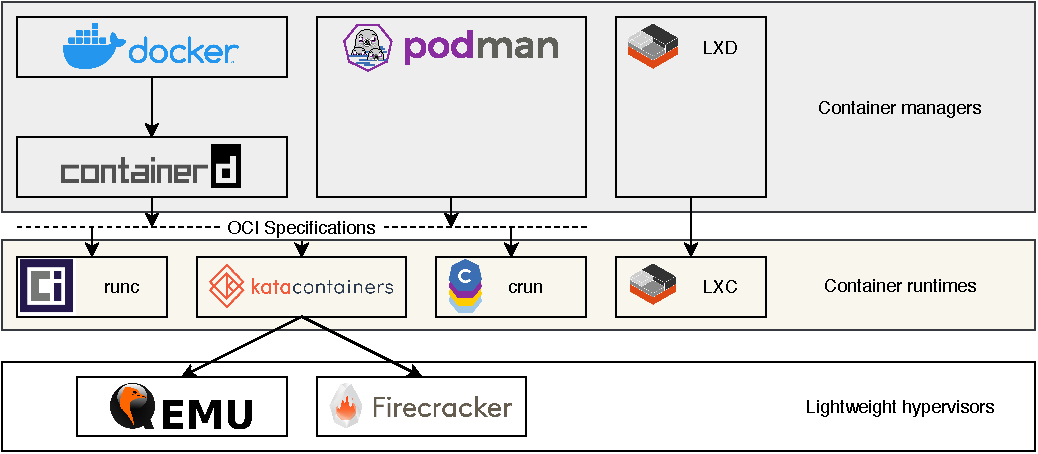
\includegraphics[width=\linewidth]{images/ecosystem.pdf}
    \caption{Small overview of the current container ecosystem}
    \label{fig:overview}
  \end{center}
\end{figure}
\paragraph{}\textbf{OCI} (Open Container Initiative) is "an open governance structure for the express purpose of creating open industry standards around container formats and runtime."\cite{oci} They currently have two specifications: the format of the image that has to be given to an OCI compatible runtime, and the commands to interact with such runtime.

\section{Containerisation solutions}
\paragraph{}\textbf{Docker}\cite{merkel2014docker} is today probably the most known container manager solution for containerization.  Since its apparition in 2014, its interest in the PaaS sector has not ceased to grow.  It consists of a daemon, running on the host, which allows us to easily manage different containers.  It relies on Containerd, "An industry-standard container runtime with an emphasis on simplicity, robustness and portability"\cite{containerd}, which is a more complete container runtime than what I presented before, with embedded network management, storage driver management, and other mechanisms.  Containerd is not meant to be used standalone though, which is why we still use Docker.  By default, Docker uses \texttt{runc} as container runtime but is compatible with any runtime that fulfills the OCI\cite{oci} requirements.

The main advantages of Docker are its simplicity of use, its production-grade quality, the huge fleet of ready-to-run containers publicly available and a lot of useful tools (like \texttt{docker-swarm} that come along with it).  This is the solution currently used by INGInious.

\paragraph{}"\textbf{Podman} is a daemonless container engine for developing, managing, and running OCI\cite{oci} Containers on your Linux System."\cite{podman}  Podman presents itself as a viable true alternative to Docker.  Its main difference is the fact that it runs daemonless, it runs containers as detached child processes and containers can be rootless by default (while it is only a recent feature coming up to Docker).  It can also manage pods, which are groups of containers deployed on the same machine. Its default runtime is \texttt{runc} as well.  Podman is an Open-Source project and is still growing a lot, the latest version at this day (2020-05-30) is v1.9.3, released 8 days ago, and already 797 commits have been done since then!

\paragraph{}"\textbf{LXC} is a userspace interface for the Linux kernel containment features."\cite{lxc}  This solution is developed and maintained by Canonical Ltd.  Docker used to be based on LXC until it created its own execution environment.  LXC came out recently with a new solution; LXD, which offers about the same things as Docker does.  A bunch of ready to run images publicly available, and a nice command-line interface to interact with containers.  The only missing feature of LXD compare to Docker, regarding our use case, is the possibility to launch a container with a command and stop it when it is finished.  LXC starts a complete init process for each container, in which you can then come and execute your command.

\paragraph{}\textbf{Linux-VServer}\cite{linux-vserver} is a bit of a special one.  No namespaces are used to provide isolation here, they rely on contexts to separate multiple virtualized systems.  They have modified the Linux kernel to provide some utilities like process isolation, network isolation and CPU isolation.  The main advantage of this approach is scalability as it can run a large number of containers, the drawback is the portability.  It requires a modified version of the kernel and it also misses some features like checkpoint and resumes that we can have with more classical containerization and real virtualization.  This is a project much older than Docker and its contemporaries and it differs in goal.  It is not appropriate for the INGInious workload.  This is an experience more similar to what classical VM provides, where you will set up multiple applications in one environment.  The container is not built for one single purpose.

\paragraph{}\textbf{OpenVZ}\cite{openvz} is another container-based virtualisation solution.  But this time it uses namespaces to provide it.  It also has its way of dealing with system resources management, more complete than cgroup.  Even though this is more close to what runc and LXC provide in terms of isolation, this is still not the kind of experience appropriate for INGInious use case.  This is designed, as for Linux-VServer, for a more complete server experience.

\paragraph{}\textbf{Kata Containers} is not another container manager.  It is an OCI compatible runtime.  With the specificity that it does not run mainstream containers as \texttt{runc}, but lightweight virtual machines, using KVM virtualization and with Qemu (originally), Firecracker or Cloud Hypervisor (still in its early days) as the hypervisor.  Those two first currently available hypervisors are not equivalent though, as the original one has more features (like devices assignment) and the second one has a lower memory footprint and smaller attack surface (smaller codebase).
They put forward four features of their solution:
\begin{itemize}
\renewcommand\labelitemi{--}
  \item \textbf{Security}: Thanks to their virtualization solution, each runtime has its own kernel, with real network, i/o and memory isolation.
  \item \textbf{Compatibility}:  They support industry standards, as the OCI\cite{oci} and legacy virtualization technologies.
  \item \textbf{Performance}:  Their performances are consistent with classical containerization solutions.
  \item \textbf{Simplicity}:  They eliminate the need to have a virtual machine dedicated to host containers.
\end{itemize}

\paragraph{}\textbf{crun} is a complete equivalent of \texttt{runc}, yet another OCI compatible runtime, but this one is implemented in C, which give it a small performance advantage over \texttt{runc}, implemented in GO.  \texttt{crun} has also full support for cgroupv2, which is still lacking for \texttt{runc} for the time being (2020-04-22).

\paragraph{}With the variaty of container manager, container runtimes and storage drivers, we can compose many different solutions.  Those are presented later, in Chapter 4.  Here is a quick summary of the different elements I presented here:

\begin{center}
\begin{tabular}{|l|l|c|c|}
  \hline
  \textbf{Name} & \textbf{Tool type} & \textbf{Appropriate}\footnotemark & \textbf{OCI}\footnotemark \\
  \hline
  \hline
  Docker & Container manager & Y & Y\\
  Podman & Container manager & Y & Y\\
  LXD & Container manager & Y & N\\
  \hline
  Linux-VServer & Container \textit{hypervisor} & N & N \\
  OpenVZ & Container \textit{hypervisor} & N & N \\
  \hline
  LXC & Container runtime & Y & N \\
  runc & Container runtime & Y & Y \\
  crun & Container runtime & Y & Y \\
  Kata Containers & Container runtime & Y & Y \\
  \hline
\end{tabular}
\end{center}
\footnotetext[1]{Could be use with INGInious}
\footnotetext[2]{Comply with the OCI specifications}
